%%%%%%%%%%%%%%%%%%%%%%%%%%%%%%%%%%%%%%%%%%%%%%%%%%%%%%%%%%%%%%%%%%%%%%
%%%%%%%%% Select one of the options, and comment the rest of them

%%%%%%%%%% Option 1:  to compile with pdflatex : parameter "t" - to align to the top
\documentclass[professionalfonts,t]{beamer}
%sans font?

%%%%%%%%%% Option 3: to create handout for print
%\documentclass[t,handout]{beamer}
%\usepackage{pgfpages}              % to put several slides on one page
%\pgfpagesuselayout{2 on 1}[a4paper, border shrink=5mm]             % 2 slides on 1 page
%\pgfpagesuselayout{4 on 1}[a4paper,landscape, border shrink=5mm]   % 4 slides on 1 page, and landscaped


%%%%%%%%%%%%%%%%%%%%%%%%%%%%%%%%%%%%%%%%%%%%%%%%%%%%%%%%%%%%%%%%%%%%
%%%%%%%%%%%%%% Select the Theme %%%%%%%%%%%%%%%%%%%%%%%%%%%%%%%%%%%
\usetheme{Dresden}     % OK
%\usetheme{Berlin}
%\usetheme{Bergen}      % NO
%\usetheme{Boadilla}    % NO
%\usetheme{Copenhagen}  % NO
%\usetheme{Hannover}    % NO
%\usetheme{Luebeck}     % NO
%\usetheme{Marburg}     % NO
%\usetheme{Pittsburgh}  % NO
%\usetheme{default}
%\usetheme{Singapore}   % OK
%\usetheme{boxes}
%\usecolortheme{structure}
%\usecolortheme{rose}
%\usecolortheme{beaver}


\definecolor{mymaroon}{cmyk}{0.0, 1.0, 1.0, 0.498}
\definecolor{myblue}{cmyk}{1.0, 1, 0, 0.5}
\definecolor{mygreen}{cmyk}{100, 0, 100, 50}
\setbeamercolor*{palette secondary}{use=structure,fg=white,bg=myblue}
\setbeamercolor*{palette tertiary}{use=structure,fg=white,bg=mymaroon}

%\usepackage{beamerthemesplit}              %
\beamertemplateballitem % fancy bullets and numbering

\setbeamertemplate{navigation symbols}{}   % suppress navigation symbols
\addtobeamertemplate{frametitle}{}{%
	\iffalse
	
	\begin{tikzpicture}[remember picture,overlay]
	\node[anchor=center, yshift=-13pt, xshift=-5pt] at (current page.north) 
	{\includegraphics[height=1.1cm]{../images/ANL_black}\hspace{10cm}};
	
	\node[anchor=north east, yshift=3pt, xshift=0pt] at (current page.north east) 
	{
\includegraphics[height=0.7cm]{../images/IIT_Logo_blk}};
	\end{tikzpicture}
    
     \fi
}
% other possibilities to include LOGO. it puts it in RLC

%
%\pgfdeclareimage[width=1cm]{logo}{../images/IIT_Logo}
%\logo{\pgfuseimage{logo}}


% load additional packages
\usepackage{xcolor}
\usepackage{graphicx}
\usepackage{amsmath}
\usepackage{amssymb}
\usepackage{amsthm}
\usepackage{graphicx}
\usepackage{url}
\usepackage{color}
\usepackage{booktabs} % Allows the use of \toprule, \midrule and \bottomrule in tables
\usepackage{pifont}% http://ctan.org/pkg/pifont
\usepackage[export]{adjustbox}
\usepackage{tikz}
\usetikzlibrary{shapes.misc}
\usetikzlibrary{shapes,arrows,decorations.markings,shadows,positioning}

% Your Abbreviations
\newcommand\bE{{\mathbb{E}}}
\newcommand\bR{{\mathbb{R}}}
\newcommand\bH{{\mathbf{H}}}
% End abbreviations

\newcommand\Wider[2][3em]{%
	\makebox[\linewidth][c]{%
		\begin{minipage}{\dimexpr\textwidth+#1\relax}
			\raggedright#2
		\end{minipage}%
	}%
}

%%%%%%%%%%%%%%%%%%%%% to edit the main text below
%NOTES ON SOME TECHNICS
%%%% Box %%%%%%%%%%%%%%%%%%%%%%%%%%%%%%%%%%%%%%%%%%%%%%%
%{\fbox{ \parbox[t]{10cm}{ SOME TEXT }}}

%%% include a picture. The file should be with extention EPS, e.g. FILENAME.EPS
%\begin{figure}[h]
%\centering
%\includegraphics[width=.7\linewidth]{FILENAME}
%\caption{{\footnotesize PUT_CAPTION }}
%\end{figure}

%\subtitle{}
%\institute[ANL/IIT]{Argonne National Laboratory\\Illinois Institute of Technology}

\title[Space Charge 2017]{Study of space charge dominated beams at the AWA rf photoinjector}
\author[N.Neveu]{{\Large Nicole Neveu}}
\institute[ANL, IIT] % (optional, but mostly needed)
{   Illinois Institute of Technology \\
	Argonne National Laboratory \\
    \url{nneveu@anl.gov} 
}
% - Use the \inst command only if there are several affiliations.
% - Keep it simple, no one is interested in your street address.
\date{ \today \\

\includegraphics[width=3cm,keepaspectratio]{../images/Argonne_cmyk_black}%
\hfill \hfill \hfill%
\includegraphics[width=4cm,keepaspectratio]{../images/IIT_logo}%
}

%\date[IIT, April 2009]{
%           Space Charge 2017 \\ Oc 18, 2009  }



\begin{document}


\begin{frame}
  \titlepage
\end{frame}
\begin{frame}
	\frametitle{Outline}
	\tableofcontents
\end{frame}

%\begin{frame}{Outline of the talk}
%  \tableofcontents
%  % You might wish to add the option [pausesections]
%\end{frame}


% Structuring a talk is a difficult task and the following structure
% may not be suitable. Here are some rules that apply for this
% solution:

% - Exactly two or three sections (other than the summary).
% - At *most* three subsections per section.
% - Talk about 30s to 2min per frame. So there should be between about
%   15 and 30 frames, all told.

% - A conference audience is likely to know very little of what you
%   are going to talk about. So *simplify*!
% - In a 20min talk, getting the main ideas across is hard
%   enough. Leave out details, even if it means being less precise than
%   you think necessary.
% - If you omit details that are vital to the proof/implementation,
%   just say so once. Everybody will be happy with that.

\section{Facility Introduction}
%%%%%%%%%%%%%%%%%%%%%%%%%%%%%%%%%%%%%%%%%%%%%%%%%%%%%%%%%%%%%%%%%%%%%%%%%%%%%%%%
\subsection{Photoinjectors}
\begin{frame}[t]
\frametitle{AWA Facility}
\begin{columns}[T] % align columns
	\begin{column}{.48\textwidth}
		%\color{red}\rule{\linewidth}{4pt}		
		
			Two photocathode guns and accompanying linacs:
			\begin{itemize}
				\item{\underline{\textbf{Drive Line}}: $Cs_2Te$ cathode, 6 linac cavities}
				\begin{itemize}
					\item{Charge 0.1-100nC}
					\item{Energy $\leq$ 65 MeV}
					
				\end{itemize}
				\item{\underline{\textbf{Witness Line}}: $Mg$ cathode, 1 linac cavity}
				\begin{itemize}
					\item{Charge 0.1-10nC}
					\item{Energy $\leq$ 15 MeV}
				\end{itemize}
			\end{itemize}
	\end{column}%
	\hfill%
	\begin{column}{.48\textwidth}
		%\color{blue}\rule{\linewidth}{4pt}
		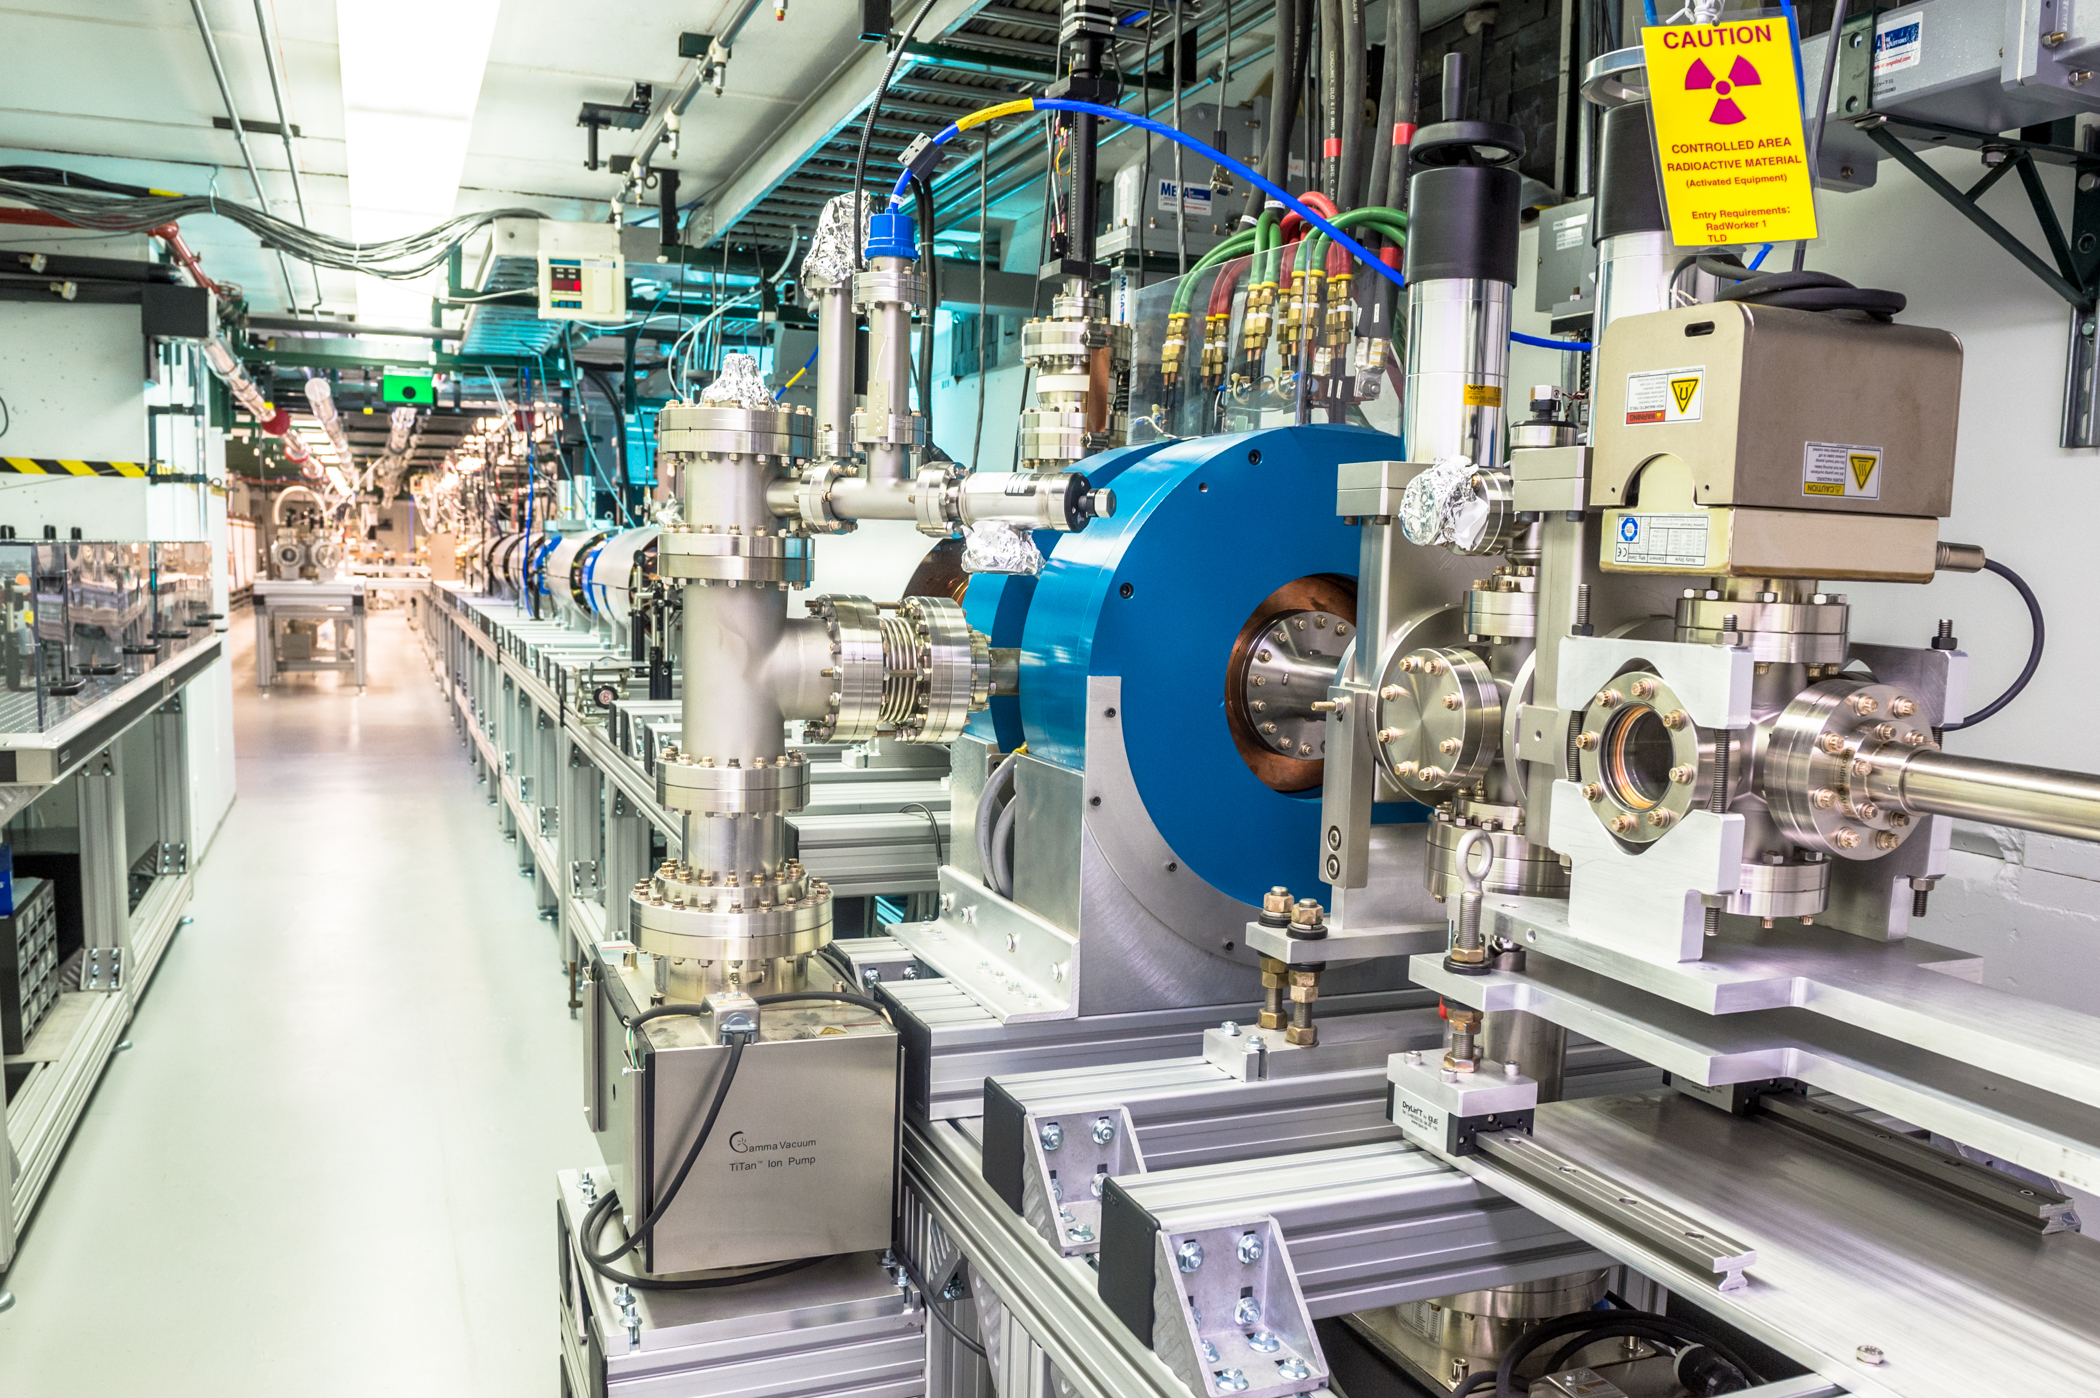
\includegraphics[width=1.0\linewidth, right]{../images/drive_gun}
	\end{column}%
\end{columns}
\end{frame}
%%%%%%%%%%%%%%%%%%%%%%%%%%%%%%%%%%%%%%%%%%%%%%%%%%%%%%%%%%%%%%%%%%%%%%%%%%%%%%%%
\subsection{Ongoing Experiments}
\begin{frame}[t]
	\frametitle{AWA Facility}
	\vspace{-1em}
	Current experiments include:
	\begin{itemize}
		\item{Two Beam Acceleration (TBA)}
		\item{Beam line design for TBA = my thesis}
		\item{Dielectric accelerating and decelerating structure tests}	
	\end{itemize}
    \vspace{1em}
    % for trim = left, lower, right, upper
	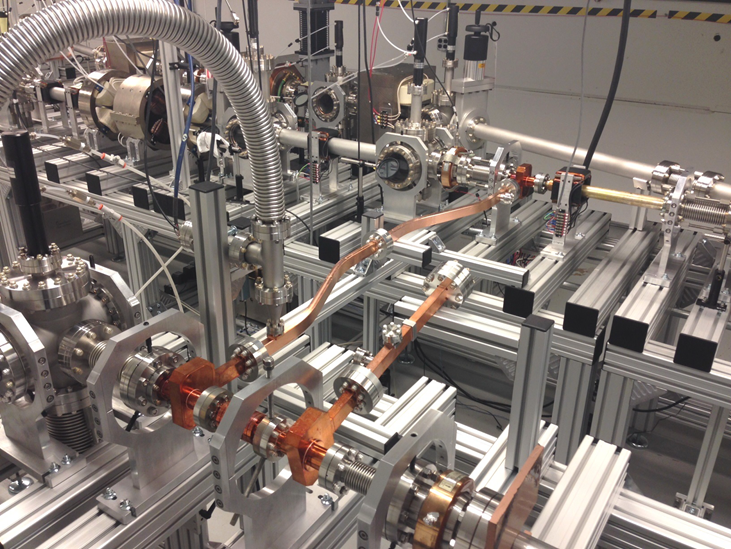
\includegraphics[width=0.5\linewidth, trim={0 0 0 1.65cm},clip]{../images/stage}\hfill%
	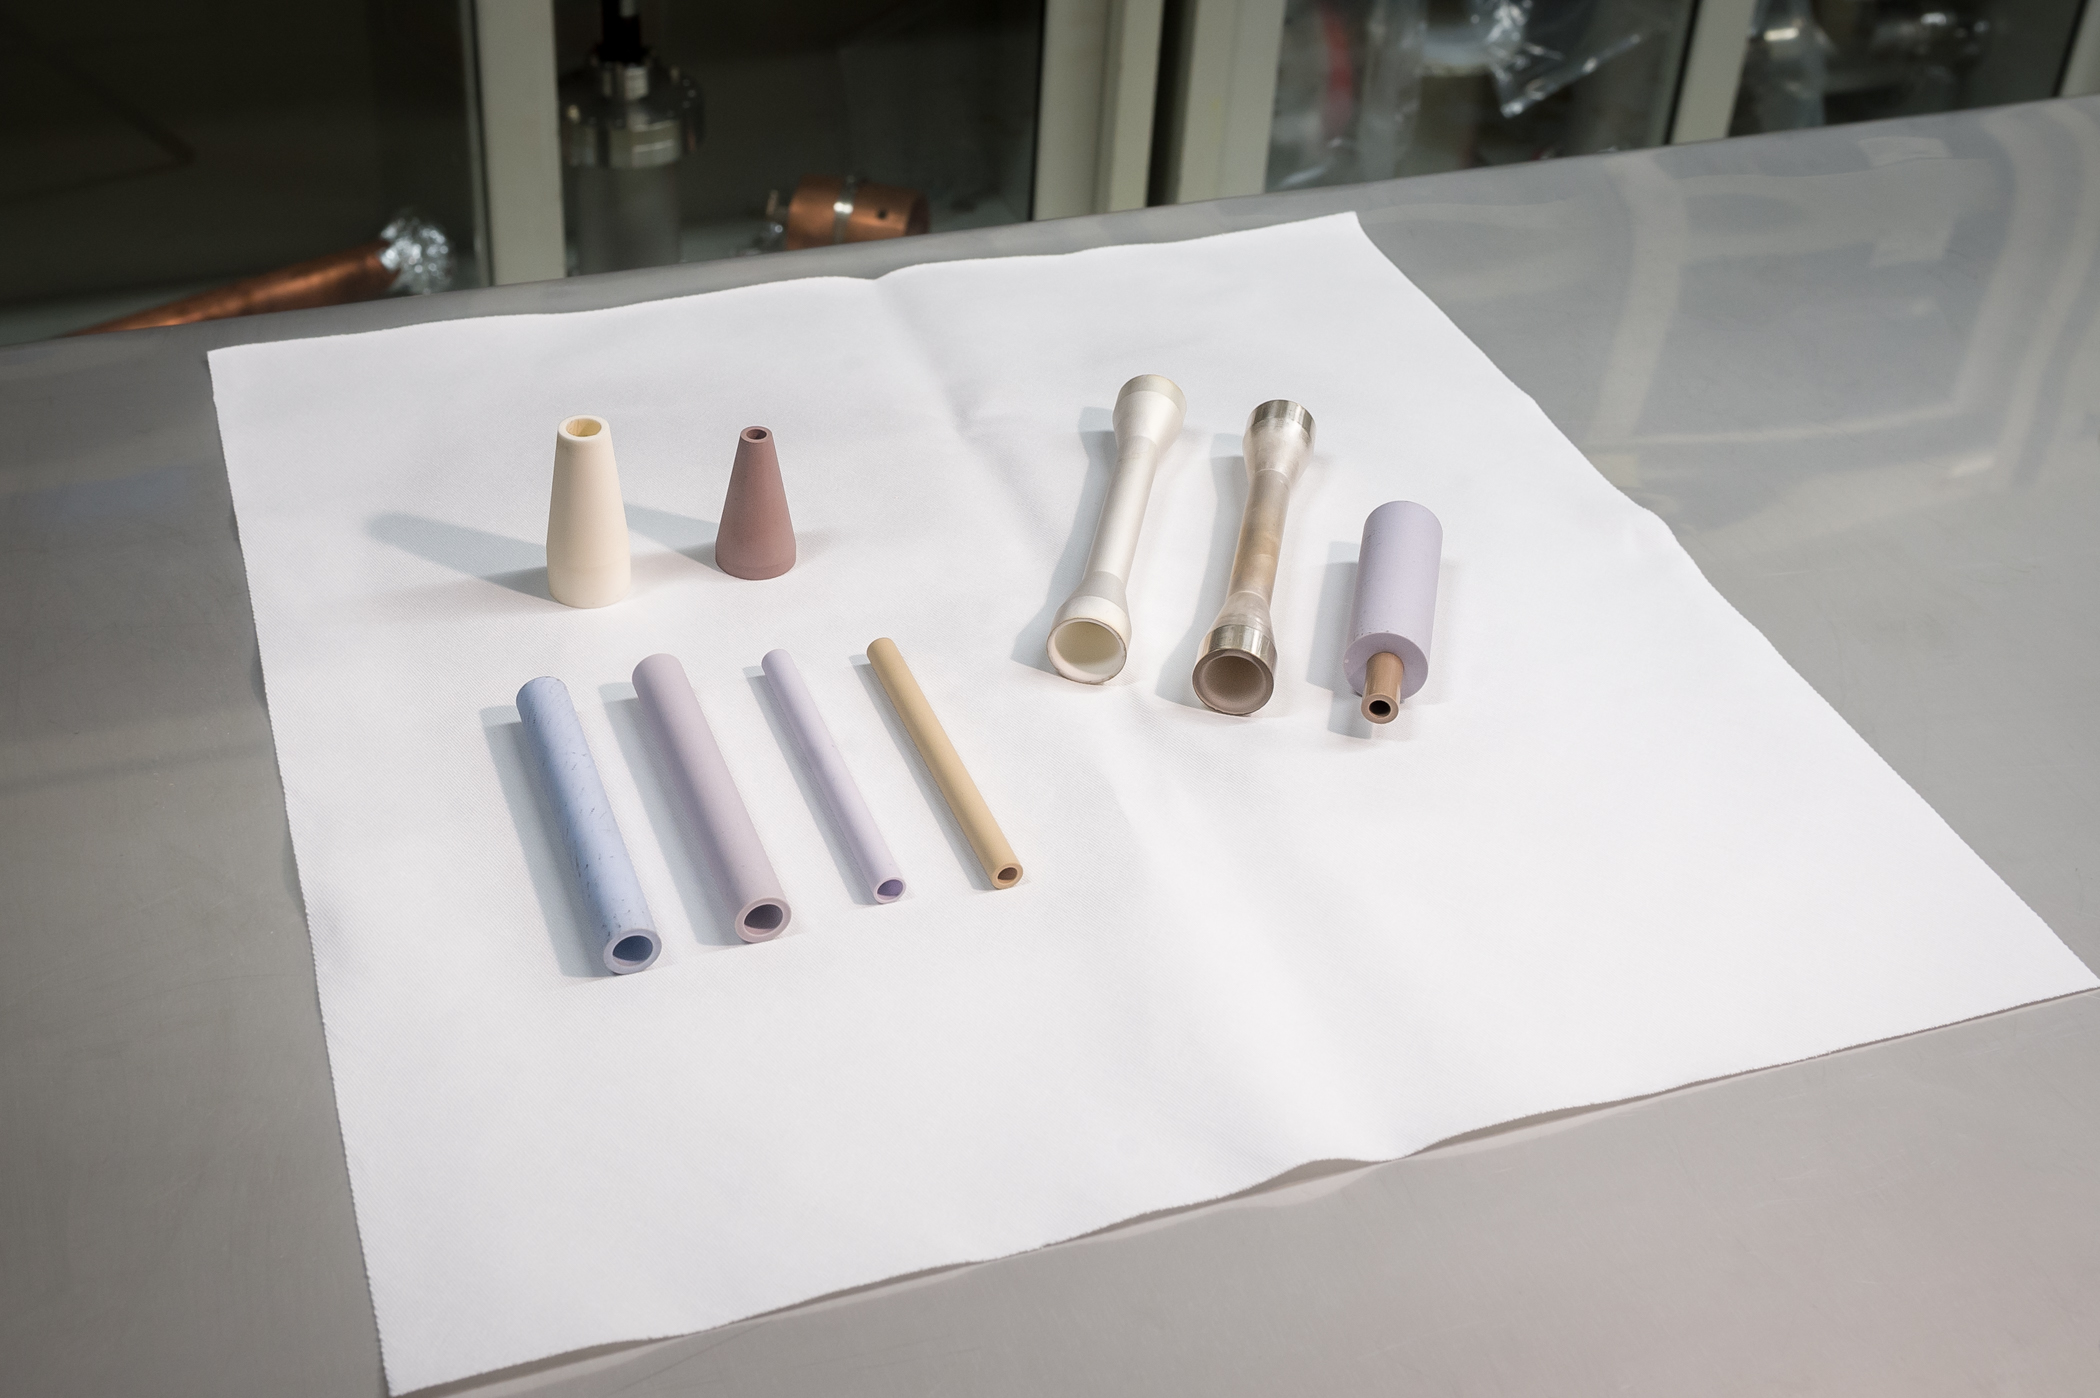
\includegraphics[width=0.5\linewidth]{../images/dielectrics}	
\end{frame}
%%%%%%%%%%%%%%%%%%%%%%%%%%%%%%%%%%%%%%%%%%%%%%%%%%%%%%%%%%%%%%%%%%%%%%%%%%%%%%%%
\begin{frame}
	\frametitle{AWA Facility}
	\vspace{-1em}
Current experiments include:
\begin{itemize}
	\item{Emittance Exchange (EEX)}
	\item{Electron Radiography Imaging (ERI)}
	\item{Cathode Studies}
\end{itemize}
\vspace{0.3cm}
\centering
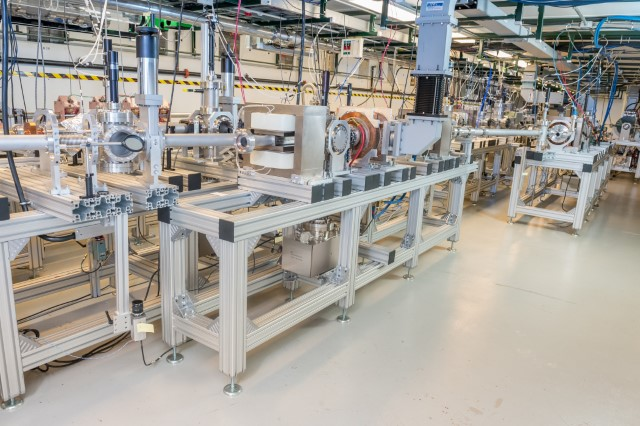
\includegraphics[width=0.5\linewidth]{../images/EEX}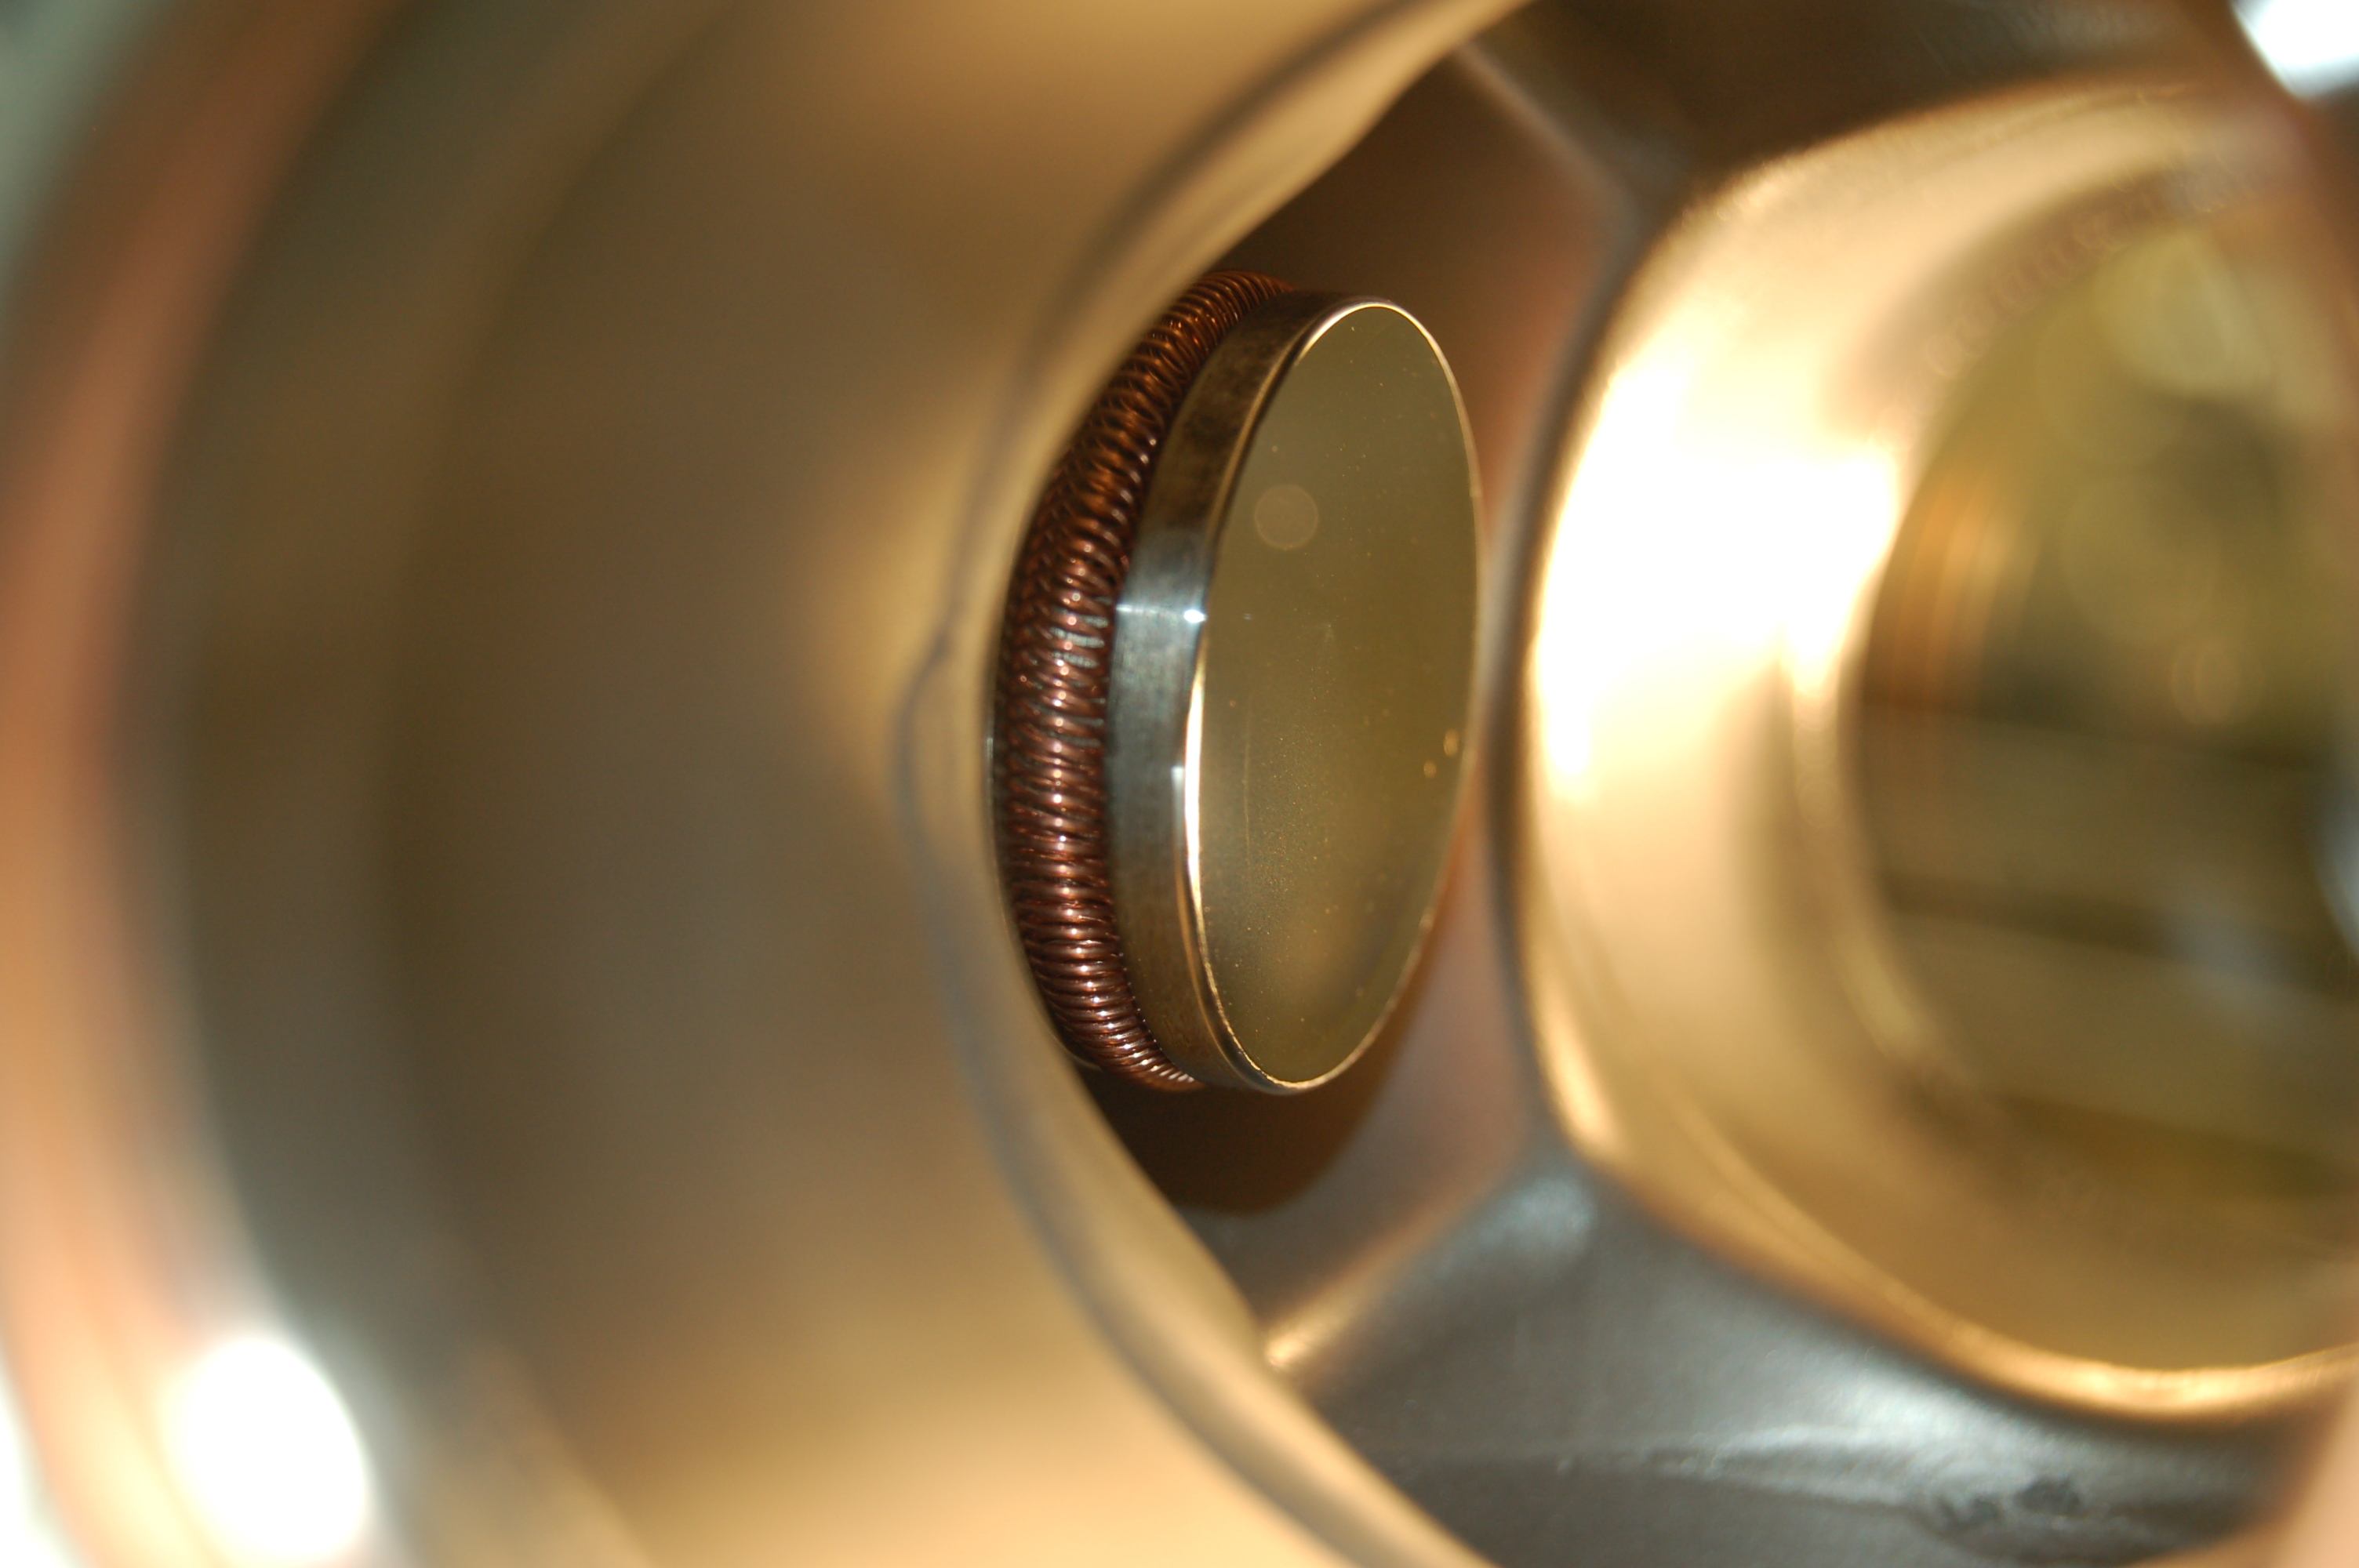
\includegraphics[width=0.5\linewidth]{../images/cathode1}
\end{frame}
%%%%%%%%%%%%%%%%%%%%%%%%%%%%%%%%%%%%%%%%%%%%%%%%%%%%%%%%%%%%%%%%%%%%%%%%%%%%%%%%
\section{Simulations}
\subsection{Code}
\begin{frame}[containsverbatim]{Select the Theme/ColorTheme}
\begin{verbatim}
\usetheme{Dresden}      %\usetheme{Berlin}
%\usetheme{Luebeck}     %\usetheme{Marburg}
%\usetheme{Pittsburgh}  %\usetheme{default}

%\usecolortheme{structure} %\usecolortheme{rose}
\usecolortheme{beaver}
\end{verbatim}

\begin{itemize}
\item And many more. Read the manual.
\item {\bf Rule of Thumbs: Simple is better.}
\item A math presentation should be a math presentation and
not a slide-show for Vouge or Glamour Magazine.
\end{itemize}
\end{frame}
%%%%%%%%%%%%%%%%%%%%%%%%%%%%%%%%%%%%%%%%%%%%%%%%%%%%%%%%%%%%%%%%%%%%%%%%%%%%%%%%
\subsection{High Charge}
\begin{frame}[containsverbatim]{Cover Slide}


\end{frame}
%%%%%%%%%%%%%%%%%%%%%%%%%%%%%%%%%%%%%%%%%%%%%%%%%%%%%%%%%%%%%%%%%%%%%%%%%%%%%%%%
\begin{frame}[containsverbatim]

Make fancy numbering and bullets:
\begin{verbatim}
    \beamertemplateballitem
\end{verbatim}

\smallskip

Nice splitting of the sections and subsections \begin{verbatim}
    \usepackage{beamerthemesplit}
\end{verbatim}

\begin{block}{Summary}
Put something in a block
\end{block}

\begin{verbatim}
    \begin{block}{Summary}
    Put something in a block
    \end{block}
\end{verbatim}

\end{frame}
%%%%%%%%%%%%%%%%%%%%%%%%%%%%%%%%%%%%%%%%%%%%%%%%%%%%%%%%%%%%%%%%%%%%%%%%%%%%%%%%

\begin{frame}[containsverbatim]{Blocks, Theorems, Examples}

\begin{beamerboxesrounded}[shadow=true]{Theorem}
Prove that $x^n+y^n=z^n$.
\end{beamerboxesrounded}

\begin{example}
For example $3^2+4^2=5^2$
\end{example}

\begin{verbatim}
    \begin{beamerboxesrounded}[shadow=true]{Theorem}
    Prove that $x^n+y^n=z^n$.
    \end{beamerboxesrounded}

    \begin{example}
    For example $3^2+4^2=5^2$
    \end{example}
\end{verbatim}
\end{frame}
%%%%%%%%%%%%%%%%%%%%%%%%%%%%%%%%%%%%%%%%%%%%%%%%%%%%%%%%%%%%%%%%%%%%%%%%%%%%%%%%
\begin{frame}{Transition}

Pause command
\begin{itemize}
\pause \item One Step
\pause \item Two
\pause \item The end.
\end{itemize}

Or More complicated (not necessarily better)\pause

\begin{enumerate}
\item<5-6> Beatles
\item<6-7>  Pick Floyd
\item<-7> Led Zeppelin
\item<-8>  Lenon
\end{enumerate}
\end{frame}
%%%%%%%%%%%%%%%%%%%%%%%%%%%%%%%%%%%%%%%%%%%%%%%%%%%%%%%%%%%%%%%%%%%%%%%%%%%%%%%%
\begin{frame}[containsverbatim]{The code}
\begin{verbatim}
Pause command
\begin{itemize}
\pause \item One Step
\pause \item Two
\pause \item The end.
\end{itemize}

Or More complicated (not necessarily better)\pause

\begin{enumerate}
\item<5-6> Beatles
\item<6-7>  Pick Floyd
\item<-7> Led Zeppelin
\item<-8>  Lenon
\end{enumerate}

\end{verbatim}
\end{frame}
%%%%%%%%%%%%%%%%%%%%%%%%%%%%%%%%%%%%%%%%%%%%%%%%%%%%%%%%%%%%%%%%%%%%%%%%%%%%%%%%
\section{Experimental Measurements}
\subsection{Beam Size Measurements}
\begin{frame}{Finally}
\begin{block}{Remark}
Avoid complicated overlays and too much animation. Usually ``pause'' is more than enough.
\end{block}
\bigskip
Other overlay commands: ONLY, UNCOVER, INVISIBLE, ALT,

\pause
\begin{center}
\bigskip
{\Large  The End \\[.5cm] Good Luck with your slides!}
\end{center}
\end{frame}
%%%%%%%%%%%%%%%%%%%%%%%%%%%%%%%%%%%%%%%%%%%%%%%%%%%%%%%%%%%%%%%%%%%%%%%%%%%%%%%%
\end{document}